%% LaTeX Template for ISIT 2023
%%
%% by Stefan M. Moser, June 2022
%% 
%% derived from bare_conf.tex, V1.4a, 2014/09/17, by Michael Shell
%% for use with IEEEtran.cls version 1.8b or later
%%
%% Support sites for IEEEtran.cls:
%%
%% https://www.michaelshell.org/tex/ieeetran/
%% https://moser-isi.ethz.ch/manuals.html#eqlatex
%% https://www.ctan.org/tex-archive/macros/latex/contrib/IEEEtran/
%%

\documentclass[conference,a4paper]{IEEEtran}


%% depending on your installation, you may wish to adjust the top margin:
\addtolength{\topmargin}{9mm}
%% apart from this
%% *** do not adjust lengths that control margins, column widths, etc.! ***
%% *** do not use packages that alter fonts (such as pslatex)!          ***

%%%%%
%% Packages:
\usepackage[utf8]{inputenc} 
\usepackage[T1]{fontenc}
\usepackage{url}              % provides \url{...}
%\usepackage{ifthen}          % provides \ifthenelse
\usepackage{cite}             % improves presentation of citations

\usepackage[cmex10]{amsmath}  % Use the [cmex10] option to ensure complicance
                              % with IEEEXplore (see bare_conf.tex)
\interdisplaylinepenalty=1000 % As explained in bare_conf.tex
\usepackage{mleftright}       % fix to wrong spacing of \left-,
\mleftright                   % \middle- \right-commands 

\usepackage{graphicx}         % provides \includegraphics{...} to
                              % include graphics (pdf format)
\usepackage{booktabs}         % fixes poor spacing in tables and
                              % provides \toprule, \midrule, \bottomrule

%\usepackage{algorithmicx}    % provides an algorithmic environment for
                              % describing algorithms. See
                              % https://ctan.org/pkg/algorithmicx

% \usepackage[caption=false,font=footnotesize]{subfig}
                              % provides subnumbering within a
                              % floating figure or table

%% For arrays and multiple-line equations, use the
%% IEEEeqnarray-environment. See
%%              https://moser-isi.ethz.ch/manuals.html#eqlatex  
%% for instructions.

%% Do NOT use amsthm or hyperref!
%% -IEEEtran provides its own versions of theorems.
%% -IEEEXplore does not accept submissions with hyperlinks


%%%%%
%% correct bad hyphenation here
\hyphenation{op-tical net-works semi-conduc-tor}
\usepackage{amsthm}
\usepackage{amsfonts}

\DeclareMathOperator{\dist}{dist}
\def\E{\mathbb{E}}
\def\R{\mathbb{R}}
\def\d{\mathrm{d}}
\newtheorem{lemma}{Lemma}
\newtheorem{example}{Example}
\newtheorem{definition}{Definition}
\newtheorem{theorem}{Theorem}
% -------------------------------------------------------------------------

\begin{document}

\title{On the Sample Complexity of High Dimensional Learning with Interpolation of Dataset}

%%%%%%
\author{%
  \IEEEauthorblockN{Anonymous Authors}
  %\IEEEauthorblockA{%
  %  Please do NOT provide authors' names and affiliations\\
  %  in the paper submitted for review, but keep this placeholder.\\
  %  ISIT23 follows a \textbf{double-blind reviewing policy}.}
}

%%%%%% Please only add the author names and affiliations for the FINAL
%%%%%% version of the paper, but NOT for the paper submitted for review!
%
%%%%%
%%%%% Single author, or several authors with same affiliation:
% \author{%
%   \IEEEauthorblockN{Stefan M.~Moser}
%   \IEEEauthorblockA{ETH Zürich\\
%                     8092 Zürich, Switzerland\\
%                     moser@isi.ee.ethz.ch}
%                   }
%
%%%%%
%%%%% Several authors with up to three affiliations:
% \author{%
%   \IEEEauthorblockN{Stefan M.~Moser}
%   \IEEEauthorblockA{ETH Zürich\\
%                     ISI (D-ITET), ETH Zentrum\\
%                     8092 Zürich, Switzerland\\
%                     moser@isi.ee.ethz.ch}
%   \and
%   \IEEEauthorblockN{Albus Dumbledore and Harry Potter}
%   \IEEEauthorblockA{Hogwarts School of Witchcraft and Wizardry\\
%                     Hogwarts Castle\\ 
%                     1714 Hogsmeade, Scotland\\
%                     \{dumbledore, potter\}@hogwarts.edu}
% }
%
%%%%%   
%%%%% Many authors with many affiliations:
% \author{%
%   \IEEEauthorblockN{Albus Dumbledore\IEEEauthorrefmark{1},
%                     Olympe Maxime\IEEEauthorrefmark{2},
%                     Stefan M.~Moser\IEEEauthorrefmark{3}\IEEEauthorrefmark{4},
%                     and Harry Potter\IEEEauthorrefmark{1}}
%   \IEEEauthorblockA{\IEEEauthorrefmark{1}%
%                     Hogwarts School of Witchcraft and Wizardry,
%                     1714 Hogsmeade, Scotland,
%                     \{dumbledore, potter\}@hogwarts.edu}
%   \IEEEauthorblockA{\IEEEauthorrefmark{2}%
%                     Beauxbatons Academy of Magic,
%                     1290 Pyrénées, France,
%                     maxime@beauxbatons.fr}
%   \IEEEauthorblockA{\IEEEauthorrefmark{3}%
%                     ETH Zürich, ISI (D-ITET), ETH Zentrum, 
%                     CH-8092 Zürich, Switzerland,
%                     moser@isi.ee.ethz.ch}
%   \IEEEauthorblockA{\IEEEauthorrefmark{4}%
%                     National Yang Ming Chiao Tung University (NYCU), 
%                     Hsinchu, Taiwan,
%                     moser@isi.ee.ethz.ch}
% }
%

\maketitle

%%%%%
%% Abstract: 
%% If your paper is eligible for the student paper award, please add
%% the comment "THIS PAPER IS ELIGIBLE FOR THE STUDENT PAPER
%% AWARD." as a first line in the abstract. 
%% For the final version of the accepted paper, please do not forget
%% to remove this comment!
%%
\begin{abstract}
  This paper estimates the sample complexity for interpolation in high dimensional space.
  To be specific, we model the learning task as interpolation of convex hull consisting of i.i.d. sampled data
  , and the sample complexity is the number of training data which guarantees that
  the probability measure of the convex hull
  tends to one. It is shown that the sample complexity has exponential relationship with the feature dimension for various distribution families
  considered in this paper, which sheds insight on the difficulty of  high dimensional learning in a general sense. 
\end{abstract}


\section{Introduction}
\label{sec:intro}
In machine learning, intuitively we model a learning task as interpolating the
training data. Under such interpretation, we are prone to think that state-of-the-art
algorithms work well in high dimensional space because the models can interpolate training data well. 
However, Balestriero et al. \cite{balestriero2021learning}
argues that this is a misconception and the interpolation almost surely never occurs in high-dimensional spaces.
Their logic is as follows: assuming the training data follows a certain distribution. Take $N$ samples from such a distribution
and consider whether the new or ($N+1$)-th sample falls in the convex hull of the first $N$ samples. 
Under certain conditions they find that the new sample falls outside with high probability.
In their terminology, the interpolation occurs whenever a new sample belongs to the convex hull of previous samples.
By citing previous theoretical studies on this ideal geometric statistical model and extensive simulation,
they justify their assertion on why interpolation almost surely never occurs.
Further experiments on other real dataset \cite{yousefzadeh2022extent} also show that
test dataset mostly fall out of the
convex hull of training dataset and augment the statement of Balestriero.

Following the geometric statistical model described above, we can derive the sample size which makes
interpolation almost surely occurs.
This sample size, or sample complexity, can be used to evaluate the task difficulty for a given distribution
and dimension before the computational extensive experiments.
Technically speaking the sample complexity is obtained when we let the sample size and the dimension tend to infinity simultaneously and
then investigate the condition under which the interpolation error converges to zero.
In our work, we give
an asymptotic upper bound of the interpolation error and then obtain the sample complexity of the interpolation in
high dimensional learning.
We show that when the training data are sampled from polynomial,
exponential and truncated distribution families,
we need exponentially large number of samples for vanishing interpolation error.
Due to the exponential dependency of the sample size on the dimension, we recommend dimension reduction or feature extraction
before applying machine learning model. Besides the relationship between the sample size $N$ and the dimension $d$,
we also reveal the dependency of $N$ on the decaying rate of the distribution.

The study of interpolation error $p_{N,d}$ is closely related with the quantity $\E[F_N]$,
the expectation of the number of facets of the convex hull. Loosely speaking,
the inequality relationship $p_{N,d} \leq \frac{\E[F_N]}{Nd}$ holds. Therefore, the asymptotic
value of $\E[F_N]$ gives an upper bound of $p_{N,d}$.
The study of $\E[F_N]$
is an old topic in stochastic geometry. As far as we know, the recent advance dates back to Dwyer's work on the estimation of $\E[F_N]$,
in which the order of $\E[F_N]$ about $N$ is obtained \cite{dwyer1991convex}. In our paper, we will extend Dwyer's work
to get a more accurate asymptotic value of $\E[F_N]$ in $\R^d$.

The organization of this paper is as follows: In Section \ref{sec:int_f}, we develop a method of obtaining $\E[F_N]$ by generalizing Carnal's integration formula
% of $H(x)=P(d_{12}\geq x)$ 
from two dimensional space to higher dimensions.
In Section \ref{sec:three_distriutions}, for three different distribution families we then derive the explicit asymptotic
expressions of $\E[F_N]$ and the sufficient condition for $p_{N,d}\to 0$, as $N,d \to \infty$. The sample complexity follows from the sufficient condition
in each case.
The main contribution of this paper,
which is summarized in Section \ref{sec:conclusion},
is to give the sample complexity for the vanishing interpolation error.
We also obtain a complete integration formula for $\E[F_N]$,
and following the classification of distributions of previous authors \cite{carnal1970konvexe,dwyer1991convex},
we derive the asymptotic expression
of $\E[F_N]$ for each category.

Below we define some notations to be used throughout this paper.
Without specific emphasis, all $d$-dimensional distributions considered in this paper are spherically symmetric.
Let $X=(X^{(1)},\dots, X^{(d)})$ follow such a distribution.
Then we use $F(x)=P(|X|\geq x)$ to denote the probability that a random point lies outside
a $d$-sphere ($d$-dimensional sphere centered at origin) with radius $x$.
The marginal distribution of each component of $X$ is determined by $G(x)=P(X^{(1)}\geq x)$.
Let $\dist$ represent the distance from the origin to the hyperplane spanned by $X_1, \dots, X_d$.
Specifically, in 2-D, the hyperplane is the straight line passing through $X_1$ and $X_2$.
We use $H(x)=P(\dist\geq x)$ to denote the probability that $\dist$ is larger than $x$.
When $n$ tends to infinity, the functions $f(n)$ and $g(n)$ are asymptotic equivalent if $\lim_{n\to \infty} \frac{f(n)}{g(n)}=1$.
We denote this relationship as $f(n) \sim g(n)$.

\section{Related work}
Since the interpolation error is bounded by
asymptotic value of $\E[F_N]$,
in this section we give a brief overview on the topic of studying $\E[F_N]$.

The asymptotic expression of $\E[F_N]$ as $N\to \infty$
was studied initially by R{\'e}nyi and Sulanke \cite{renyi1963konvexe}.
They considered
bivariate Gaussian distribution and uniform distribution
in a planar convex region.
Following the derivation of R{\'e}nyi, for $d=2,3$, Efron \cite{efron1965convex} obtained the explicit integration formula for $\E[F_N]$ and $p_{N,d}$ 
when samples follow Gaussian distribution or uniform distribution within a unit sphere.
Later on,  R{\'e}nyi's work was generalized by
Carnal \cite{carnal1970konvexe}, who
classified symmetric 2-D distributions
into three categories according to their tails:
polynomial, exponential, and truncated tails.
Then he obtained the asymptotic expression of $\E[F_N]$
for each category of distributions.




The study of $\E[F_N]$ for $d>2$ was made firstly by
Raynaud
\cite{raynaud1970enveloppe}.
He obtained the asymptotic formula of $\E[F_N]$
for uniform distribution in a hyperball
and standard Gaussian distribution in $\mathbb{R}^d$.
Afterwards, following Carnal, Dwyer \cite{dwyer1991convex}
estimated the order of $\E[F_N]$ about $N$
for three different distribution families.


For studies focusing on an specific distribution family,
Davis et al. \cite{davis1987convex} found the relationship
between the distributions with algebraic tails $F(x) \sim x^{-k}$ and Poisson random process.
They showed that for $k>0, d=2$,
$\mathrm{H}_N$ converges to the convex hull of a Poisson random process,
and
the limit of $\E[F_N]$ can be derived from this random process.
The special case $k=0, d=2$ is treated in a later paper, in which the
limit distribution of $F_N$ is computed \cite{aldous1991number}.

Studies related to distributions with exponential tails mainly focus on Gaussian distribution.
Kabluchko et al. \cite{kabluchko2020absorption} obtained explicit expressions for $p_{N,d}$;
Affentranger \cite{affentranger1991convex} derived $\E[F_N]$;
Hueter et al. \cite{hueter1999limit} studied the concentration property of $F_N$ and obtained
an upper bound for $\E[F_N]$ sharper than the bound in \cite{dwyer1991convex}.

For truncated tails,
Affentranger \cite{affentranger1991convex} studied one sub-category called beta-typed distribution and obtained
the asymptotic value of $\E[F_N]$.

Beside the number of facets $\E[F_N]$,
the asymptotic value of other quantities related with $\mathrm{H}_N$, such as the volume, and the surface area,
were systematically investigated in a general framework involving the property of facets
\cite{schneider2008stochastic, barany2008random}.

\section{Mathematic Models}
\label{sec:int_f}

Let $\mathcal{X}_N = \{X_1, X_2, \dots, X_N\}$ be a set of i.i.d. random points generated from
a spherically symmetric distribution in $\mathbb{R}^d$.
Let $\mathrm{H}_N$ denote the convex hull of $\mathcal{X}_N$,
and the interpolation error is defined as $p_{N,d}=P(X_{N+1} \not\in \mathrm{H}_N)$.

To study $p_{N,d} \to 0$, we introduce two additional quantities of $H_N$: the number of vertices
$V_N$ and the number of facets $F_N$.
A facet of a $d$-dimensional object is one of its $(d-1)$-dimensional faces.
Besides, 
In this paper, we study the mathematical expectation
of $F_N$, denoted as $\E[F_N]$, and we consider its asymptotic value as $N\to \infty$.

The starting point is the integration formula for $\E[F_N]$.
Carnal \cite{carnal1970konvexe}
obtained
this formula for 2-D distributions,
which is given as follows:
\begin{align}
     \E[F_N] &= \binom{N}{2} \int_0^{\infty} 
     \left[G(x)^{N-2} + (1-G(x))^{N-2} \right]|\mathrm{d} H(x)| 
     \label{eq:E_F_N_2_d}
\end{align}
The integration formula of $\E[F_N]$ involves the function $G(x)$ and $H(x)$,
whose definitions are given at the end of Section \ref{sec:intro}.
Both functions are expressed with $F(x)$ in the following way:
\begin{align}
   G(x) &=\frac{1}{\pi} \int_x^{\infty}\arccos\frac{x}{y} |\mathrm{d} F(y)| \\
     H(x) &= \frac{2}{\pi} \int_x^{\infty} \arccos \frac{x}{y} |\mathrm{d}(F^2(y))|
     \label{eq:H_expression_2_dim}
\end{align}
For $d\geq 2$ and $N\geq d+1$, the formula is given as
\begin{align}
     \E[F_N] &= \binom{N}{d} \int_0^{\infty} 
     \left[G(x)^{N-d} + (1-G(x))^{N-d} \right]|\mathrm{d} H(x)| 
    \label{eq:E_F_N_d}
\end{align}
Formula \eqref{eq:E_F_N_d} first appeared in the proof section of \cite{raynaud1970enveloppe}
and can further be generalized to compute other combinatorial properties of $\mathrm{H}_N$ (like surface area and volume)
\cite{barany2008random}.
Dwyer obtained the integration formula for $G(x)$ in $d\geq 2$ as:
\begin{align}\label{eq:G_d_kappa}
     G(x) & = \int_x^{+\infty} \kappa \left(\frac{x}{y} \right) |\mathrm{d}F(y)| \\
     \kappa(r) & = \frac{\Gamma(\frac{d}{2})}
     {\sqrt{\pi}\Gamma(\frac{d-1}{2})}\int_r^{1}
     (1-u^2)^{(d-3)/2}\mathrm{d}u\label{eq:kappa_r}
\end{align}
where $\kappa(r)$ is the fraction of the surface area of a unit $d$-sphere
cut off by a plane at distance $r$ from the origin.

We cannot compute $\E[F_N]$ from $F(x)$ yet, since no formula for $H(x)$ with respect to $F(x)$ is given in previous studies.
The following theorem solves this problem by giving the integration formula for $H(x)$ in $d\geq 2$:
\begin{theorem}\label{thm:H}
For $d\geq 2$, the integration formula for $H(x)$ is given as
\begin{equation}
     H(x) = \frac{2}{\pi}
     \int_x^{+\infty} \arccos\frac{x}{y}
     |\mathrm{d} (K^d(y))|\label{eq:H_expression_d_dim}
\end{equation}
where the auxiliary function $K(x)$ is defined in the following way:
\begin{align}
     \lambda_d(x)  :&=(1-x^2)^{\frac{d-2}{2}}
     \label{eq:lambda_r}\\
     K(x) :&=P\left(\sqrt{(X^{(1)})^2+(X^{(2)})^2}>x \right)\notag \\
     &=
     \int_x^{+\infty} 
     \lambda_d \left(\frac{x}{y} \right)|\d F(y)|
     \label{eq:K_x}
\end{align}
\end{theorem}
%It is easy to observe that \eqref{eq:H_expression_d_dim} reduces to 
%\eqref{eq:H_expression_2_dim} when $d=2$.
For standard Gaussian distribution in $\R^d$,
$X_1, X_2$ are independent
Gaussian random variables, and we can verify that \eqref{eq:K_x} holds with $K(x) = e^{-x^2/2}$.
In fact, $1-K(x)$ is the CDF of Rayleigh distribution.
%For general spherical distributions, the function $K(x)$ itself is irreverent with the dimension $d$.
The proof of Theorem \ref{thm:H}
is provided in Appendix \ref{app:th}.
\section{Three distribution families}\label{sec:three_distriutions}
Notice that in \eqref{eq:E_F_N_d}, $G(x)<\frac{1}{2}$ for $x>0$. Therefore the
term $G(x)^{N-d}$ decays at an exponential rate as $N-d\to \infty$.
As a result, we obtain
\begin{align}
     \E[F_N] \sim \binom{N}{d} \int_0^{+\infty} 
      (1-G(x))^{N-d} |\d H(x)| \textrm{ as } N-d\to \infty
     \label{eq:E_F_N_d_sim}
\end{align}
Let $\E[V_N]$ represent the expected number of
vertices of $\mathrm{H}_N$.
By far it is not clear whether there exist explicit relations
between $\E[F_N]$ and $\E[V_N]$
for general spherical symmetric distributions.
However, we can give some estimations by inequality.
Using Corollary 19.6 of \cite{brondsted2012introduction}, we have the following
inequality:
\begin{equation}\label{eq:F_V_upper}
     F_N \geq (d-1) V_N - (d+1)(d-2)
 \end{equation}
Combined with $p_{N,d} = \frac{\E[V_{N+1}]}{N+1}$, which comes from
\cite{efron1965convex}, we have the following upper bound for $p_{N,d}$:
\begin{equation}\label{eq:p_N_d_bound}
    p_{N,d} \leq \frac{\E[F_N]}{d N} \textrm{ as } N \gg d
\end{equation}

We use the symbol $a \gg b$ if $a$ is a function of $b$ and $\lim_{b\to \infty} \frac{a}{b} = \infty$.
Based on \eqref{eq:E_F_N_d_sim}, in the following
we derive the asymptotic expression of $\E[F_N]$
for three different distribution families.

To precisely define these distribution families, we introduce the concept of slowly varying function.
\begin{definition}
A function $L(x)$ is
slowly varying as $x\to \infty$
if for all $\lambda>0$,
$\lim_{x\to\infty}\frac{L(\lambda x)}{L(x)}=1$
holds.
\end{definition}

\subsection{Distributions with polynomial tails}

With the help of a slowly varying function $L(x)$,
distributions with polynomial tails are written
in the following form:
\begin{equation}\label{eq:F_poly_tail}
     F(x) = x^{-k} L(x), k\geq 0
\end{equation}

Dwyer\cite{dwyer1991convex} has obtained $G(x)$ as:
\begin{equation}\label{eq:g_poly_tail}
     G(x) \sim \frac{\Gamma(\frac{d}{2})}{2\sqrt{\pi} \Gamma(\frac{d-1}{2})}
     B\left(\frac{k+1}{2}, \frac{d-1}{2}\right) F(x)  \textrm{ as } x\to \infty
\end{equation}

From Theorem \ref{thm:H}, we obtain the asymptotic
expression of $H(x)$ and $\E[F_N]$, which is
summarized in the following theorem:
\begin{theorem}\label{thm:poly_tails}
     For distributions with polynomial tails defined in \eqref{eq:F_poly_tail},
     we have
\begin{equation}\label{eq:H_poly_tail_exp}
     H(x) \sim \frac{2^d \pi^{(d-1)/2}\Gamma^d(\frac{k}{2}+1)
     \Gamma(\frac{dk+1}{2})}{
         \Gamma^d(\frac{k+1}{2}) \Gamma(\frac{dk}{2}+1)} G(x)^d 
         \textrm{ as } x\to \infty
\end{equation}
and 
\begin{equation}\label{eq:efn_poly_second_deri}
    \E[F_N] \sim \frac{2^d \pi^{(d-1)/2}\Gamma^d(\frac{k}{2}+1)
    \Gamma(\frac{dk+1}{2})}{
        \Gamma^d(\frac{k+1}{2}) \Gamma(\frac{dk}{2}+1)}
        \textrm{ as } N \to \infty, d \textrm { is fixed}
\end{equation}
\end{theorem}
Equation \eqref{eq:efn_poly_second_deri} tells
us that $\E[F_N]$ converges to a constant as $N \to \infty$.
Without consideration of the actual constant, the result of
Theorem \ref{thm:poly_tails} is an refinement to Dwyer's Theorem 1 for the expected number of facets \cite{dwyer1991convex}.
When $d=2$, the result was obtained in (2.4) of \cite{carnal1970konvexe}
and Theorem 4.4 of \cite{davis1987convex}.
\begin{example}
     We consider a special case of polynomial tail called multivariate t-distribution.
     Its pdf is given by
     \begin{equation}\label{eq:pxy_student_t}
          p(x) = \frac{\Gamma((k+d)/2)}{\Gamma(k/2)(k\pi)^{d/2}}
          \left(1+\frac{1}{k}||x||^2
          \right)^{-\frac{k+d}{2}}, x \in \mathbb{R}^d
      \end{equation}
      The parameter $k$ is the degree of freedom for this distribution.
      We can obtain the radius distribution
      $F(x)$ as $F(x) \sim \frac{2\Gamma(\frac{k+d}{2})}{\Gamma(k/2)\Gamma(d/2)} k^{k/2-1} x^{-k}$.
      The marginal distribution is Student's t-distribution. To obtain $G(x)$, which is just the tail area
of the t-distribution, we use an existing asymptotic result found in \cite{andrew1976}.
\begin{equation} \label{eq:eq_dv}
    G(x) \sim k^{\frac{k}{2}-1} \frac{\Gamma \left(\frac{k+1}{2} \right)}
    {\sqrt{\pi} \Gamma\left(\frac{k}{2}\right)}x^{-k}
\end{equation}
After simplification, \eqref{eq:eq_dv} is the same as \eqref{eq:g_poly_tail}.
On the other hand, using similar techniques as (1.4) in \cite{raynaud1970enveloppe},
we can obtain the pdf of the distance of the hyperplane to the origin as
\begin{equation}\label{eq:dH_dx_t_distribution}
     \frac{\d H(x)}{\d x} =  \frac{2}{\sqrt{k} B(\frac{kd}{2},\frac{1}{2})} \left(1 + \frac{x^2}{k} \right)^{-\frac{kd+1}{2}} 
\end{equation}
From above, we get the asymptotic relation $H(x) \sim \frac{2 \Gamma(\frac{kd+1}{2}) k^{kd/2-1}}{d\sqrt{\pi} \Gamma(\frac{kd}{2})}
x^{-kd}$ as $x\to \infty$, which is equivalent to \eqref{eq:H_poly_tail_exp}.

\end{example}
From \eqref{eq:efn_poly_second_deri}, we also see that
the asymptotic value of $\E[F_N]$ is an increasing function of $d$.
As $d$ increases, from \eqref{eq:p_N_d_bound}, we need more and more $N$ to control $p_{N,d}$.
The following theorem gives an estimation on the sample complexity $N$,
which is the function of dimension $d$, the error bound $\epsilon$ and the distribution parameter $k$.
\begin{theorem}\label{thm:poly_tail_sample_complexity}
  For distributions with polynomial tails with $k>0$, given $\epsilon \in (0,1)$,
  when the following condition is satisfied
\begin{equation}\label{eq:N_c_d_3_2}
  N = \frac{c^d}{k^{1/2}d^{3/2} \epsilon}, \textrm{ where } c=\frac{\sqrt{\pi}k\Gamma(k/2)}{\Gamma(\frac{k+1}{2})}>1  
\end{equation}
the interpolation error $p_{N,d} < \epsilon$ as $d\to \infty$.
\end{theorem}
From the above theorem, to guarantee the interpolation error is no more than a given precision $\epsilon$,
we require that $N$ has exponential relationship with $d$.
The higher the dimension is, the more samples are needed.
Besides, the decaying rate of the distribution also has influence on the sample size $N$.
Since $c$ is an increasing function with $k$,
larger $k$ (faster decay) also leads to more samples.
Finally, if we treat $\epsilon$ as a function of $d$ and $\lim_{d\to\infty}\epsilon \to 0$.
Theorem \ref{thm:poly_tail_sample_complexity} implies that $\lim_{d\to\infty} p_{N,d} = 0$.
For example, we can choose $\epsilon=\frac{1}{d}$.

\begin{proof}[Proof of Theorem \ref{thm:poly_tail_sample_complexity}]
When we allow $d\to \infty$, we treat $N$ as a function of $d$.
If the condition $N/d^2 \to \infty$ is satisfied, we have
\begin{equation}\label{eq:poly_E_F_N_d_infty}
\E[F_N] \sim \sqrt{\frac{2}{\pi dk}}\left(
      \frac{\sqrt{\pi}k \Gamma(k/2)}
     {\Gamma(\frac{k+1}{2})}
 \right)^d \textrm{ for } k>0
\end{equation}
Since $N$ in \eqref{eq:N_c_d_3_2} satisfies the assumption $N/d^2 \to \infty$,
it follows from \eqref{eq:p_N_d_bound}
\begin{align*}
p_{N,d} \leq &\frac{d^{1/2}k^{1/2}}{c^d} \E[F_N]\epsilon
\leq \sqrt{\frac{2}{\pi}}\epsilon \leq \epsilon
\end{align*}
%Then the sufficient condition for $p_{N,d} \to 0$ is obtained
%from the estimation inequality \eqref{eq:p_N_d_bound},
%combined with the asymptotic expressions for polynomial distribution families in \eqref{eq:poly_E_F_N_d_infty}.
\end{proof}

\subsection{Distributions with exponential tails}
In this subsection, we first give the definition of distributions with exponential tails.
\begin{definition}
  For a radius distribution $F(x)$, if we could find
  a slowly varying function $L(x)$ such that
  $x = L(1/F(x))$, we say that the distribution has exponential tails.
\end{definition}
Following Carnal \cite{carnal1970konvexe},
we define the following utility functions:
\begin{align}
     \epsilon(s) & = s (\log (L(s)))' \label{eq:epsilon_s}\\
     v(u) &= -\frac{1}{u} \frac{1}{(\log F(u))'}    
\end{align}
The prime notation represents the symbol for differentiation. When $v(u)$ satisfies
certain regularity conditions prescribed in (2.15) of \cite{carnal1970konvexe},
we can obtain that $\epsilon(s)$ is a slowly varying function.
Dwyer \cite{dwyer1991convex} obtains the expression of $G(x)$ as:
\begin{equation}\label{eq:G_x_exp}
     G(x) \sim \frac{2^{(d-3)/2}}{\sqrt{\pi}}\Gamma\left(\frac{d}{2}\right)
     v^{(d-1)/2}(x) F(x)
      \textrm{ as } x\to \infty
\end{equation}
We make the analysis complete by giving the following theorem.
\begin{theorem}\label{thm:exponential_tails}
     Suppose there exists a slowly
     varying function $L(x)$ such that \linebreak $x=L(1/F(x))$,
     and $\epsilon(s)$ is defined in \eqref{eq:epsilon_s}, then
\begin{equation}\label{eq:H_x_exp}
     H(x) \sim \frac{\pi^{\frac{d-1}{2}} 2^{\frac{d+1}{2}}}{\sqrt{d}}v^{\frac{-d+1}{2}}(x)G^d(x)
     \textrm{ as } x\to \infty
\end{equation}
 and
 \begin{equation}\label{eq:exp_e_f_n}
     \E[F_N]\sim \frac{\pi^{\frac{d-1}{2}} 2^{\frac{d+1}{2}}}{\sqrt{d}} (\epsilon(N))^{-\frac{d-1}{2}}
     \textrm{ as } N \to \infty, d \textrm { is fixed}
 \end{equation}
\end{theorem}
 Using \eqref{eq:epsilon_s}, we note that the term
 $(\epsilon(N))^{-\frac{d-1}{2}}$
 is obtained in Dwyer's Theorem 2 \cite{dwyer1991convex}.
 Our improvement on the asymptotic value of $\E[F_N]$ is that we obtain its preceding term only involving $d$.
 When $d=2$, equation \eqref{eq:exp_e_f_n} is consistent with (2.20) of \cite{carnal1970konvexe}.
 For standard $d$-dimensional Gaussian distribution, we have $L(s)=\sqrt{2\log s}$.
 From \eqref{eq:epsilon_s}, $\epsilon(s) = (2\log s)^{-1}$. And we obtain from \eqref{eq:exp_e_f_n}
 that $\E[F_N]\sim \frac{2^d}{\sqrt{d}}(\pi \log N)^{\frac{d-1}{2}}$,
 which is consistent with (1.11) of \cite{raynaud1970enveloppe}.

 If $d\to\infty$ and $N/d^2\to \infty$, we have
\begin{align}\label{eq:d_infty_exp_E_F_N}
      \E[F_N]\sim \frac{\pi^{\frac{d-1}{2}} 2^{\frac{d+1}{2}}}{\sqrt{d}} \epsilon(N)^{\frac{-d+1}{2}}
\end{align}

Similar to the analysis of polynomial tails, we obtain the
sufficient condition for $p_{N,d} \to 0$ from
\eqref{eq:p_N_d_bound} and \eqref{eq:d_infty_exp_E_F_N}.
\begin{theorem}\label{thm:exp_tails_sample}
  For distributions with exponential tails, given $\epsilon \in (0,1)$, when the following condition is satisfied
  \begin{equation}\label{N_d_relationship_exp_tail}
    N\cdot \epsilon(N)^{(d-1)/2} = \frac{\pi^{\frac{d-1}{2}} 2^{\frac{d+1}{2}}}{d^{3/2} \epsilon},
  \end{equation}
  the interpolation error $p_{N,d} < \epsilon$ as $d\to \infty$.
\end{theorem}
For any given $d$, we can obtain $N$ from the implicit relationship in \eqref{N_d_relationship_exp_tail}.
When $d\to \infty$, \eqref{N_d_relationship_exp_tail} implies $N\to \infty$.
To better illustrate Theorem \ref{thm:exp_tails_sample},
we consider an special exponential distribution of the form $F(x) \sim C(k)\exp(-x^k)$, we obtain from \eqref{eq:epsilon_s}
that $\epsilon(s)=(k\log s)^{-1}$.
Then from Theorem \ref{thm:exp_tails_sample},
we can estimate that
$N$ grows faster than $c^d$ for any constant $c$ but slower than $\exp(d^2)$.
Besides, $N$ increases with $k$ for fixed $d$.
In other words, larger $k$ (faster decay) leads to more samples.

\subsection{Distributions with truncated tails}
In this subsection, let $L(x)$ also represent a slowly varying function, and we consider the distribution which satisfies
the following conditions:
\begin{equation}\label{eq:F_truncated}
     F(1-x) \sim x^k L\left(\frac{1}{x} \right)  \text{ as } x \to 0^+, k> 0,
     F(x) = 0 \text{ for } x \geq 1
\end{equation}
In \eqref{eq:F_truncated}, $x \to 0^+$ means that $x\to 0$ from the right hand side of $0$.

As mentioned by Dwyer \cite{dwyer1991convex}, uniform distribution
in the unit ball satisfies \eqref{eq:F_truncated} with
$F(1-x) \sim d\cdot x$.

After simplification of (4.1) in \cite{dwyer1991convex}, we obtain
\begin{align}
    G(1-x) \sim a
    L\left(\frac{1}{x} \right)
    x^{k+\frac{d-1}{2}} \textrm{ as } x \to 0^+ 
    \label{eq:truncated_G_1_x}
\end{align}
where
\begin{align}
a &=\frac{2^{\frac{d-1}{2}} k \Gamma(\frac{d}{2})}
    {(d-1) \sqrt{\pi} \Gamma(\frac{d-1}{2})}
    B\left(k, \frac{d+1}{2}\right) \notag \\
    &= \frac{2^{\frac{d-3}{2}} k \Gamma(\frac{d}{2})\Gamma(k)}
    {\sqrt{\pi} \Gamma\left(k+\frac{d+1}{2}\right)}
    \label{eq:a}
\end{align}
Below, we give the theorem in regards to the asymptotic value of $H(1-x)$ and $\E[F_N]$:
\begin{theorem}\label{thm:truncated_tails}
     For distributions with truncated tails
     defined in \eqref{eq:F_truncated},
     we have
\begin{align}
     H(1-x)  \sim b
     L^d(1/x) x^{d(k+\frac{d}{2}-1)+\frac{1}{2}} 
     \textrm{ as } x \to 0^+ \label{eq:truncated_H_1_x}
\end{align}
where
\begin{align}
     b =  \frac{k^d}{\pi}
     2^{\frac{1}{2} + d(\frac{d}{2}-1)} B^d\left(k, \frac{d}{2}\right)
     B\left( \frac{1}{2},
     d\left(k+\frac{d}{2} -1 \right)+1 \right)
     \label{eq:b}
 \end{align}
When $N\to \infty$ and $d$ is fixed, we have
 \begin{align}\label{eq:efn_truncated_formula}
     \E[F_N] \sim &\frac{b}{d!}a^{-d+\frac{d-1}{2k+d-1}}
     \Gamma 
     \left(d+1-\frac{d-1}{2k+d-1}\right)
     \notag\\
     &\cdot N^{\frac{d-1}{2k+d-1}}
     L(N)
     ^{\frac{d-1}{2k+d-1}}
 \end{align}
 where the parameter $a$ is defined in \eqref{eq:a}.
\end{theorem}
 The leading polynomial term $N^{\frac{d-1}{2k+d-1}}$ in \eqref{eq:efn_truncated_formula}
 is the same with that in Dwyer's Theorem 3
 but other coefficients are missing in Dwyer's result
 \cite{dwyer1991convex}. Therefore, we say that Dwyer only made the order estimation
 of $\E[F_N]$ while we obtain its asymptotic value.
 When $d=2$, equation \eqref{eq:efn_truncated_formula} reduces to (3.4) of \cite{carnal1970konvexe}.
 For uniform distribution with $k=1, L(N)=d$, we can verify that
 \eqref{eq:efn_truncated_formula} is equivalent with (1.1)
 of \cite{raynaud1970enveloppe}.
 \begin{example}\label{ex:beta_typed}
  We consider a special distribution with truncated tail called
  beta-typed distribution. Its density function is defined as:
  \begin{equation}\label{eq:pxy_beta_t}
    p(x) = \frac{\Gamma(\frac{d}{2}+ k)}{\pi^{d/2} \Gamma(k)} (1-||x||^2)^{k-1},
    ||x|| <1, x \in \mathbb{R}^d
\end{equation}
 $p(x)=0$ for $||x||\geq 1$.
 The so-called beta-typed distribution first appeared in \cite{affentranger1991convex}.
 In Equation (3.1) of Affentranger's formulation,
 he uses the symbol $q$, which has the relationship  $k=q+1$ with our symbol $k$.
 From \eqref{eq:pxy_beta_t} and \eqref{eq:F_truncated}, we can obtain
 \begin{equation}\label{eq:beta_typed_L_N}
  L(N)=\frac{2^k}{kB(d/2,k)},
 \end{equation}
 which is irrelevant with $N$.
 Besides, similar to \eqref{eq:dH_dx_t_distribution},
 we can obtain the pdf of the distance of the hyperplane to the origin as
\begin{equation}
     \frac{\d H(x)}{\d x} = \frac{2}{B(\frac{1}{2}, d(k+\frac{d}{2}-1)+\frac{1}{2})}\left(1 -x^2\right)^{d(k+\frac{d}{2}-1)-\frac{1}{2}} 
\end{equation}
From above, we get the asymptotic relation $H(x) \sim \frac{2^{\mu}}{\mu B(1/2, \mu)}
x^{\mu}$ with $\mu=d(k+\frac{d}{2}-1)+\frac{1}{2}$ as $x\to \infty$,
which is equivalent to \eqref{eq:truncated_H_1_x}.

 We can further verify that
 \eqref{eq:efn_truncated_formula} is equivalent with the expression of $c_3$
 in (3.3) of \cite{affentranger1991convex}.
 \end{example}
 When we allow $d\to \infty$ and $N/d^2 \to \infty$, we obtain
 \begin{equation}\label{eq:truncated_d_inf}
  \E[F_N] \sim 2^{\frac{d+2k}{2}}\pi^{\frac{d-2}{2}} k\Gamma(k)e^k d^{\frac{d-3}{2}-k}
  N^{\frac{d-1}{2k+d-1}} L(N)^{\frac{d-1}{2k+d-1}}
 \end{equation}

 Similar to the previous analysis, from
 \eqref{eq:p_N_d_bound} and \eqref{eq:truncated_d_inf} we obtain
 the following theorem:
 \begin{theorem}\label{thm:truncated_tails_sample}
  For distributions with truncated tails,
  given $\epsilon \in (0,1)$,
  when the following condition is satisfied
  \begin{equation}
    \frac{N^{2k/d}}{L(N)^{\frac{d-1}{2k+d-1}}}
        =\frac{(2\pi)^{d/2}d^{(d-5)/2}}{\epsilon},
  \end{equation}
  the interpolation error $p_{N,d} < \epsilon$ as $d\to \infty$.
\end{theorem}
From Theorem \ref{thm:truncated_tails_sample}, as
distributions with exponential tails, we see that
the sample size $N$ also has super-exponential relationship
with $d$ for distribution with truncated tails.
To illustrate this point, we consider the beta-typed distribution introduced
in Example \ref{ex:beta_typed}.
Using \eqref{eq:beta_typed_L_N},
we obtain that $N(d)$
grows faster than $\exp(cd^2)$ for any constant $c$.

From the discussion of three kinds of tails, we see that the sample complexity of $N$ is the smallest for algebraic tails and the largest
for truncated tails. This is directly related with its convergent rate of $F(x)$.
For truncated tails, $F(x)$ becomes zero beyond the unit sphere, therefore it has the largest sample complexity.
For other two tails, the faster $F(x)$ decays, the larger $N$ becomes.

%%%%%%
%% An example of a floating figure using the graphicx package.
%% Note that \label must occur AFTER (or within) \caption.
%% For figures, \caption should occur after the \includegraphics.
%%
% \begin{figure}[htbp]
%   \centering
%   \includegraphics[width=0.3\textwidth]{myfigure}
%   % where a .pdf suffix will be assumed for pdflatex
%   \caption{Simulation results.}
%   \label{fig:sim}
% \end{figure}
%%%%%%

%%%%%%
%% An example of a double column floating figure using two subfigures.
%% (The subfig package must be loaded for this to work; uncomment the
%% corresponding line in the document header.)  The *-version of
%% figure makes the figure use both columns. The subfigure \label
%% commands are set within each subfloat command, the \label for the
%% overall figure must come after \caption.  \hfil must be used as a
%% separator to get equal spacing.
%%
% \begin{figure*}[htbp]
%   \centering
%   \subfloat[Caption of first subfigure.]{%
%     \label{fig:subfigA}
%     \includegraphics[width=4cm]{subfigcase1}}
%   \hfil
%   \subfloat[Caption of second subfigure.]{%
%     \label{fig:subfigB}
%     \includegraphics[width=4cm]{subfigcase1}}  
%   \caption{Two figures showing something.}
%   \label{fig:subfigures}
% \end{figure*}
% We refer to the Figures~\ref{fig:subfigA} and \ref{fig:subfigB} within
% Figure~\ref{fig:subfigures}.
%%%%%% 

%%%%%%
%% An example of a floating table.
%% Note that the \caption command should come BEFORE the table. Table
%% text will default to \footnotesize as IEEE normally uses this
%% smaller font for tables.  The \label must come after \caption as
%% always. The following example relies on booktabs.sty to fix poor
%% spacing within tables and using \toprule, \midrule, and \bottomrule
%% as proper replacement for the corresponding \hline
%%
% \begin{table}[htbp]
%   \centering
%   \caption{Recursion given by Lloyd's algorithm for the case of a
%     Gaussian random variable represented by four values.}
%   \label{tab:gaussfour}
%   \begin{IEEEeqnarraybox}[\IEEEeqnarraystrutmode%
%     % \IEEEeqnarraystrutsizeadd{2pt}{1pt}% uncomment for more spacing
%     ]{l"l"l}
%     \toprule
%     \hat{x}_1 & \hat{x}_2 & \theta \\
%     \midrule
%     0.5 & 1 & 0.75 \\      
%     0.3578 & 1.3288 & 0.8433 \\
%     0.3973 & 1.4011 & 0.8992 \\
%     0.4202 & 1.4450 & 0.9326 \\
%     0.4336 & 1.4714 & 0.9525 \\
%     0.4414 & 1.4872 & 0.9643 \\
%     0.4461 & 1.4966 & 0.9714 \\
%     0.4488 & 1.5022 & 0.9755 \\
%     \vdots && \\
%     0.4528 & 1.5104 & 0.9816 \\
%     \bottomrule
%   \end{IEEEeqnarraybox}
% \end{table}
%%%%%%



\section{Conclusion}
\label{sec:conclusion}
In this paper, we derive the sample complexity to interpolate
the convex hull of i.i.d. samples. Our work gives the sufficient
condition for the convergence of the interpolation error to zero.
Further study on the necessary condition is still an open problem.
As a byproduct, we get the asymptotic value of the number of facets
in three categories of distributions, which can also be applied
to other fields such as estimation of time complexity of algorithms
for constructing a representation of convex hulls.

%%%%%%
%% To balance the columns at the last page of the paper use this
%% command somewhere at the top of the first column of the last page:
%%
% \enlargethispage{-5cm} 
%%
%% where the exact amount of page reduction has to be adapted to the
%% actual situation.
%%
%% If the balancing should occur in the middle of the references, use
%% the following trigger:
%%
% \IEEEtriggeratref{3}
%%
%% which triggers a \newpage (i.e., new column) just before the given
%% reference number. Note that you need to adapt this if you modify
%% the paper. The "triggered" command can be changed if desired:
%%
% \IEEEtriggercmd{\enlargethispage{-20cm}}
%%
%%%%%%

%%%%%%
%% References:
%% We recommend the usage of BibTeX:
%%
\bibliographystyle{IEEEtran}
\bibliography{exportlist.bib}
%\bibliography{definitions,bibliofile}
%%
%% where we here have assume the existence of the files
%% definitions.bib and bibliofile.bib.
%% BibTeX documentation can be obtained at:
%% http://www.ctan.org/tex-archive/biblio/bibtex/contrib/doc/
%%%%%%
%% Or you use manual references (pay attention to consistency and the
%% formatting style!):



%%%%%% 
%% Appendix:
%% If needed a single appendix is created by
%%
\appendix
%%
%% If several appendices are needed, then the command
%%
% \appendices
%%
%% in combination with further \section-commands can be used.
%%%%%%

\subsection{Proof of Theorem \ref{thm:H}}\label{app:th}
\begin{lemma}\label{lem:F_0}
     Let $F_0$ represent the
probability that the distance from the origin to the straight line
$X_1X_2$ is larger than $x$, where $X_1, X_2$ follow the distribution with $F(x)=P(|X|\geq x)$.
Then 
\begin{align}\label{eq:F_0_expression}
     F_0(x)=&\frac{2\Gamma(\frac{d}{2})}
     {\sqrt{\pi}\Gamma(\frac{d-1}{2})}
     \int_x^{\infty} |\d F(y)|
     \int_x^{y} |\d F(z)| 
     \notag\\
     &\cdot \int_{a_2/z}^{a_1 /z} (1-u^2)^{\frac{d-3}{2}} \d u
 \end{align}
where
\begin{align}
     a_1 & =\frac{x^2}{y}+\sqrt{z^2-x^2}\sqrt{1-\frac{x^2}{y^2}} > 0
     \label{eq:a_1} \\
a_2 & =\frac{x^2}{y}-\sqrt{z^2-x^2}\sqrt{1-\frac{x^2}{y^2}} < 0
\label{eq:a_2}
\end{align}
\end{lemma}
Lemma \ref{lem:F_0} gives the integration formula for $P(d_{12}\geq x)$ in $\R^d$.
The geometric meaning of $a_1, |a_2|$ is illustrated in Figure
\ref{fig:a1a2}. That is, if we assume
\begin{equation}\label{eq:theta_1_theta_2}
     \cos\theta_1=\frac{x}{z}
     \textrm{ and } \cos\theta_2=\frac{x}{y} 
\end{equation}
then
\begin{equation}\label{eq:a_1_a_2}
     \frac{a_1}{z} = \cos(\theta_2 - \theta_1),
     \quad
     \frac{a_2}{z} = \cos(\theta_2+\theta_1)           
\end{equation}

\begin{figure}[!ht]
     \centering
     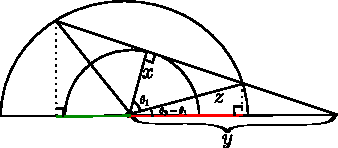
\includegraphics[width=0.8\linewidth]{dessin.pdf}
     \caption{The length of red line represents $a_1$ while the green line corresponds to $|a_2|$.}
     \label{fig:a1a2}
\end{figure}
When $d=2$, using $\int \frac{\d x}{\sqrt{1-x^2}} = -\arccos x + C$,
we obtain
$$
F_0(x)=\frac{4}{\pi} \int_x^{\infty} \arccos\frac{x}{z}|\d F(y)|
\int_x^{y} |\d F(z)|\d z
$$
which is the same with \eqref{eq:H_expression_2_dim}.
\begin{proof}[Proof of Lemma \ref{lem:F_0}]
For $d\geq 2$ and $x<z<y$, we follow the geometric approach
which is adopted to derive
$H(x)$ in \cite{carnal1970konvexe}.
Then we only need to compute the ratio of surface area
on the sphere with radius $z$. This is the area between
two planes at distance $\frac{a_1}{z}$ and $\frac{a_2}{z}$
respectively on the unit sphere. From (1.1) of \cite{dwyer1991convex},
this ratio equals $\kappa(\frac{a_2}{z}) - \kappa(\frac{a_1}{z})$
where $\kappa$ is defined in \eqref{eq:kappa_r}.

\end{proof}
To show 
$K(x) = \int_x^{+\infty} \lambda_d(\frac{x}{y})|\d F(y)|$
in \eqref{eq:K_x},
we only need to connect $\lambda_d(r)$ with its geometric meaning,
which is given in the following lemma:
\begin{lemma}
     The ratio of surface area on a unit $d$-sphere,
     satisfying $x_1^2+x_2^2\geq r$ is $\lambda_d(r)$,
     defined in \eqref{eq:lambda_r}.
\end{lemma}
\begin{proof}
     Following \cite{dwyer1991convex}, we use $\kappa_d = 2\pi^{d/2}/\Gamma(d/2)$
     to represent the surface area of the unit $d$-sphere. Then
     \begin{align*}
          \lambda_d(r) &=\frac{2}{\kappa_d} 
          \int_{\substack{x_1^2+x_2^2\geq r^2\\
          x_1^2+\dots+x_{d-1}^2\leq 1 }} 
          \frac{\d x_1 \dots \d x_{d-1}}{\sqrt{1-x_1^2-\dots -x_{d-1}^2}} \\
      &= \frac{4\pi}{\kappa_d} \int_r^1 x\d x \\
      &\cdot\int_{x_3^2+\dots + x_{d-1}^2 \leq 1-x^2} \frac{\d x_3\dots \d x_{d-1}}
      {\sqrt{1-x^2-x_3^2-\dots -x_{d-1}^2}} \\
      &=\frac{4\pi \kappa_{d-3}}{\kappa_d} \int_r^1 x\d x \int_0^{\sqrt{1-x^2}} \frac{y^{d-4}\d y}{\sqrt{1-x^2-y^2}}\\
      &=\frac{4\pi \kappa_{d-3}}{\kappa_d} \int_0^{\sqrt{1-r^2}} y^{d-4}\d y \int_r^{\sqrt{1-y^2}} \frac{x\d x}{\sqrt{1-x^2-y^2}}\\
      &=\frac{4\pi \kappa_{d-3}}{\kappa_d} \int_0^{\sqrt{1-r^2}} y^{d-4}\sqrt{1-r^2-y^2} \d y\\
      &=\frac{4\pi \kappa_{d-3}}{\kappa_d}  \frac{B(\frac{3}{2 }, \frac{d-3}{2})}{2}(1-r^2)^{(d-2)/2}\\
      &=  (1-r^2)^{(d-2)/2}
      \end{align*}
\end{proof}

\begin{lemma}\label{lem:cn_integration}
For $0<c<1$ and $n$ is a non-negative positive integer, we have
\begin{align}
    &\int_0^{c}
    [\frac{1}{(1-t)^{n+1}}+\frac{1}{(1+t)^{n+1}}]
    (c^2- t^2)^{(n-1)/2}\d t\notag\\
    &=B(\frac{n+1}{2}, \frac{1}{2})
    \frac{c^n}{(1-c^2)^{(n+1)/2}}\label{eq:c_int_eq}
    \end{align}
\end{lemma}
\begin{proof}[Proof of Lemma \ref{lem:cn_integration}]
     When $n=0$, the left hand side equals
     \begin{align*}
          \int_0^c \frac{2}{(1-t^2)\sqrt{c^2-t^2}} \d t
          = \int_0^{\sqrt{c}} \frac{1}{(1-t) \sqrt{t} \sqrt{c^2-t} }\d t
     \end{align*}     
     We make change of variables $x=\sqrt{t/(c^2-t)}$ and obtain
     the value $\frac{\pi}{(1-c^2)^{1/2}}$, which equals
     the right hand side.
     When $n=1$, we can use integration directly
     to show that \eqref{eq:c_int_eq} holds.

     Let
\begin{equation}\label{eq:f_n_c_def}
h(n,c)=   \int_0^{c}
    [\frac{1}{(1-t)^{n+1}}+\frac{1}{(1+t)^{n+1}}]
    (c^2- t^2)^{(n-1)/2}\d t
\end{equation}
When $n\geq 2$, by integration by parts 
we have 
\begin{equation}\label{eq:tmp_n_u_d_f_n}
    \frac{n}{n-1}h(n,c)
    =\int_0^{c}
    \left[\frac{1}{(1-t)^{n}}
    -\frac{1}{(1+t)^{n}}
    \right]
    t(c^2- t^2)^{(n-3)/2}
    \d t
\end{equation}
Let $t=\frac{(1+t)-(1-t)}{2}$ in the right hand side
of \eqref{eq:tmp_n_u_d_f_n}, then
\begin{align}
    \frac{2n}{n-1}h(n,c)
&=    -h(n-2,c)  
\notag\\
&+ \int_0^{c}
\left[\frac{1+t}{(1-t)^{n}}
+\frac{1-t}{(1+t)^{n}}
\right]
(c^2- t^2)^{(n-3)/2}
\d t
\end{align}
On the other hand,
From \eqref{eq:f_n_c_def},
$(c^2-t^2)^{(n-1)/2}
=[(c^2-1)+(1-t^2)](c^2-t^2)^{(n-3)/2}$
\begin{align}
    h(n, c) =& \frac{c^2-1}{2c}\frac{2}{n-1}\frac{\partial h(n,c)}{\partial c}\notag\\
    &+  \int_0^{c}
    \left[\frac{1+t}{(1-t)^{n}}
    +\frac{1-t}{(1+t)^{n}}
    \right]
    (c^2- t^2)^{(n-3)/2}
    \d t
\end{align}
Therefore,
\begin{equation}\label{eq:sim_1tc}
    h(n,c)=\frac{c^2-1}{2c}\frac{2}{n-1}\frac{\partial h(n,c)}{\partial c}
    + [2\frac{n}{n-1} h(n,c) + h(n-2, c)]
\end{equation}
then we can use induction and solve this
first order linear ODE about $h(n,c)$.
The initial condition is $h(n,0)=0$ and
suppose
$h(n-2,c)=B(\frac{n-1}{2}, \frac{1}{2})
\frac{c^{n-2}}{(1-c^2)^{(n-1)/2}}$.
Then \eqref{eq:sim_1tc} is simplified as
\begin{equation}
    \frac{\partial h(n,c)}{\partial c}
    - \frac{(n+1)c}{1-c^2} h(n,c)
    = B(\frac{n-1}{2}, \frac{1}{2})\frac{(n-1)c^{n-1}}{(1-c^2)^{(n+1)/2}}
\end{equation}
Using the integration factor $I(c)=(1-c^2)^{(n+1)/2}$, we obtain
\begin{equation}\label{eq:f_n_c_expression}
    h(n,c)= B(\frac{n+1}{2}, \frac{1}{2})
    \frac{c^n}{(1-c^2)^{(n+1)/2}}
\end{equation}

\end{proof}

Having defined $K(x), F_0(x)$, we find the following relationship holds:
\begin{lemma}\label{lem:K_F_relationship}
\begin{equation}\label{eq:F_0_integration}
     \int_u^{+\infty}
     (1-\frac{u^2}{x^2})^{\frac{d-3}{2}} |\d F_0(x)| = K^2(u)
\end{equation}
\end{lemma}
\begin{proof}[Proof of Lemma \ref{lem:K_F_relationship}]
     By the chain rule, from \eqref{eq:a_1_a_2} we obtain
\begin{align*}
    \frac{\d}{\d x}\frac{a_1}{z} &
    = \sin(\theta_2 - \theta_1)
    \left(\frac{-1}{z\sin\theta_1}
    +\frac{1}{y\sin \theta_2}\right)\\
    \frac{\d}{\d x}\frac{a_2}{z} &
    = \sin(\theta_2 + \theta_1)
    \left(\frac{1}{z\sin\theta_1}
    +\frac{1}{y\sin \theta_2}\right)
\end{align*}
where $\theta_1, \theta_2$ are defined in \eqref{eq:theta_1_theta_2}.
Then from \eqref{eq:F_0_expression}
\begin{align*}
    \frac{\d F_0(x)}{\d x}  =\frac{2\Gamma(\frac{d}{2})}
    {\sqrt{\pi}\Gamma(\frac{d-1}{2})}
    \int_x^{+\infty} |\d F(y)| \int_x^y |f(x,y,z)| |\d F(z)| 
\end{align*}
where
\begin{align*}
    f(x,y,z) &= \sin^{d-2} (\theta_2 - \theta_1)
    \left(\frac{-1}{z\sin\theta_1}
    +\frac{1}{y\sin \theta_2}\right) \\
    &- \sin^{d-2}(\theta_1 + \theta_2)
    \left(\frac{1}{z\sin\theta_1}
    +\frac{1}{y\sin \theta_2}\right)
\end{align*}
Comparing $\d F_0(x)$
with the expression of $K(x)$ in
\eqref{eq:K_x},
we only need to prove
\begin{align}
    \frac{2\Gamma(\frac{d}{2})}
    {\sqrt{\pi}\Gamma(\frac{d-1}{2})}
    \int_u^z (1-\frac{u^2}{x^2})^{\frac{d-3}{2}}
    |f(x,y,z)|\d x &=
    2(1-\frac{u^2}{y^2})^{\frac{d-2}{2}} \notag\\
    &\cdot (1-\frac{u^2}{z^2})^{\frac{d-2}{2}}
    \label{eq:ref_prove_integration}    
\end{align}
We can expand $f(x,y,z)$ as follows:
\begin{align*}
-f(x,y,z)=&\frac{\sin^{d-2}(\theta_2+\theta_1)
+ \sin^{d-2}(\theta_2 - \theta_1)}{z\sin\theta_1}\\
&+\frac{\sin^{d-2}(\theta_2+\theta_1)
- \sin^{d-2}(\theta_2 - \theta_1)}{y\sin\theta_2} \\
=&\frac{2}{z\sin\theta_1}\sum_{k \textrm{ is even}}
\binom{d-2}{k} (\sin\theta_2\cos\theta_1)^{d-2-k}\\
&\cdot(\cos\theta_2 \sin\theta_1)^k \\
+&\frac{2}{y\sin\theta_2} \sum_{k \textrm{ is odd}}
\binom{d-2}{k} (\sin\theta_2\cos\theta_1)^{d-2-k}\\
&\cdot(\cos\theta_2 \sin\theta_1)^k
\end{align*}
Therefore,
\begin{align*}
|f(x,y,z)|
&= \frac{2x^{d-2}}{y^{d-2}z^{d-2}}
\Big[
     \\
    &\sum_{k \textrm{ is even}}
    \binom{d-2}{k} (z^2-x^2)^{\frac{k-1}{2}}(y^2-x^2)^{\frac{d-2-k}{2}}\\
    &+ \sum_{k \textrm{ is odd}}
    \binom{d-2}{k}    (z^2-x^2)^{\frac{k}{2}}
    (y^2-x^2)^{\frac{d-3-k}{2}}
\Big]
\end{align*}
Let $a=z^2-u^2, b=y^2-u^2$, then
\begin{align*}
     &\int_u^z (1-\frac{u^2}{x^2})^{\frac{d-3}{2}}
     |f(x,y,z)|\d x
     =\frac{1}{y^{d-2}z^{d-2}}
     \int_0^a x^{\frac{d-3}{2}}\Big[ \\
     &\sum_{k \textrm{ is even}}
     \binom{d-2}{k} (a-x)^{\frac{k-1}{2}}
     (b-x)^{\frac{d-2-k}{2}}\\
     &+ \sum_{k \textrm{ is odd}}
     \binom{d-2}{k} (a-x)^{\frac{k}{2}}
     (b-x)^{\frac{d-3-k}{2}}
     \Big]\d x\\
     &=\frac{1}{2y^{d-2}z^{d-2}}
     \int_0^a x^{\frac{d-3}{2}}\\
     &\cdot\Big[\frac{(\sqrt{b-x} + \sqrt{a-x})^{d-2}+(\sqrt{b-x} - \sqrt{a-x})^{d-2}}{\sqrt{a-x}}\\
     &+\frac{(\sqrt{b-x} + \sqrt{a-x})^{d-2}-(\sqrt{b-x} - \sqrt{a-x})^{d-2}}{\sqrt{b-x}}\Big] \d x
\end{align*}
Let $t=\sqrt{\frac{a-x}{b-x}}$, we then obtain
\begin{align*}
     &\int_u^z (1-\frac{u^2}{x^2})^{\frac{d-3}{2}}
     |f(x,y,z)|\d x= \frac{(b-a)^{\frac{d-1}{2}}}{y^{d-2}z^{d-2}}\\
     &\cdot\int_0^{\sqrt{a/b}}
     \left[\frac{1}{(1-t)^{d-1}}+\frac{1}{(1+t)^{d-1}}\right](a-bt^2)^{\frac{d-3}{2}}\d t
\end{align*}
Let $c=\sqrt{a/b}$ and $n=d-2\geq 0$ in the expression of $h(n,c)$ in \eqref{eq:f_n_c_expression},
we obtain
\begin{align}
     \int_u^z (1-\frac{u^2}{x^2})^{\frac{d-3}{2}}
     |f(x,y,z)|\d x
     =& \frac{1}{y^{d-2}z^{d-2}}h(d-2, \sqrt{a/b}) \notag\\
     &\cdot(1-c^2)^{\frac{n+1}{2}}b^{\frac{n}{2}}\label{eq:int_u_x_f_x}
\end{align}
After simplification of \eqref{eq:int_u_x_f_x}, we obtain \eqref{eq:ref_prove_integration}.
\end{proof}

\begin{proof}[Proof of Theorem \ref{thm:H}]
     
We use $\dist(P_1,\dots, P_{d-1})$ to represent
the distance from the origin to the hyperplane passing $P_1,P_2,\dots, P_{d-1}$,
and let $F_1(x)=P(\dist(P_1,\dots, P_{d-1})\linebreak\geq x)$.


Firstly we show that $F_1(x)=K^{d-1}(x)$.
For $d=2$, it is trivial.
By induction we suppose that $F_1(x)=K^{d'-1}(x)$ is true for
$d'\leq d-1$.
Since $d'\leq d$,
the function $K(x)=P(\sqrt{(X^{(1)})^2 + (X^{(2)})^2} \geq x)$
only depends on $d$,
not on $d'$.
Therefore, in $d'$-dimensional space,
from \eqref{eq:K_x} we have $
P(\dist(P_1, \dots, P_{d'-1})\geq x) = \int_{x}^{\infty} K^{d'-2}(x)\lambda_{d'}(x/y)|\d F(y)|
$.
Then the conditional probability $P(\dist(P_1,\dots, P_{d'-1})\geq x \Big\vert |OP_1|=y)
=K^{d'-2}(x)\lambda_{d'}(x/y)$.
For $d$-dimensional space, 
we firstly specify a straight line passing through $P_{d-2}P_{d-1}$,
the space perpendicular 
to this line has $d'=d-1$ dimension while the straight line shrinks to a single point $P'$
in this subspace. Since
$P(\dist(P_1,\dots,P_{d-3},P')\geq x \Big\vert |OP'|=y)=
K^{d-3}(x)\lambda_{d-1}(x/y)$,
we have
\begin{align*}
    F_1(x) = \int_x^{+\infty} K^{d-3}(x) \lambda_{d-1}(\frac{x}{y})|\d F_0(y)|
\end{align*}
From Lemma \ref{lem:K_F_relationship} we obtain $F_1(x) = K^{d-1}(x)$.

To finish the proof and compute $H(x)$, we first specify a hyperplane $P_2P_3\dots P_{d}$,
whose distance to the origin is $y$. The subspace perpendicular to this hyperplane is a 2-D subspace,
and this hyperplane shrinks to a point $P'$ in this 2-D subspace.
Similar to (1.9) of \cite{carnal1970konvexe}, we have
\begin{align}
     H(x) =& \frac{2}{\pi}\int_x^{+\infty}|\d F_1(y)|\notag\\
     &\cdot\left[ \int_x^y \arccos\frac{x}{z}|\d K(z)|
     +\int_y^{+\infty}\arccos\frac{x}{y} |\d K(z)|\right]\notag\\
     =&\frac{2}{\pi}\int_x^{+\infty} \arccos\frac{x}{z}
     F_1(z)|\d K(z)|\notag \\
     &+\frac{2}{\pi}\int_{x}^{+\infty} K(y)F_1(y)\arccos\frac{x}{y}|\d F_1(y)| \label{eq:H_eq_n_arccos_geometric}
 \end{align}
Using $F_1(x)=K^{d-1}(x)$,
we reduce \eqref{eq:H_eq_n_arccos_geometric} to
 $$
 H(x) = \frac{2}{\pi}\int_x^{+\infty}  \arccos\frac{x}{y}\cdot
 d\cdot  K^{d-1}(y) |\d K(y)|
 $$
 which is exactly \eqref{eq:H_expression_d_dim}.
 
\end{proof}
\subsection{Proof of Theorem \ref{thm:poly_tails}}
The techniques used in this subsection are similar to the derivation of $G(x)$
in (2.3) of \cite{carnal1970konvexe}.

\begin{proof}[Proof of Theorem \ref{thm:poly_tails}]
For polynomial tails defined in \eqref{eq:F_poly_tail},
we first compute the asymptotic value of $K(x)$
as follows:
\begin{align*}
     K(x) & = \int_x^{\infty} (1-\frac{x^2}{y^2})^{\frac{d-2}{2}} |\d F(y)| \\
     &= (d-2)\int_x^{\infty} F(y)\frac{x^2}{y^3} (1-\frac{x^2}{y^2})^{\frac{d-4}{2}} \d y\\
     (y=x/t) &= (d-2)x^{-k} \int_0^{1} L(x/t) t^{k+1} (1-t^2)^{(d-4)/2}\d t \\
     & \sim F(x) \frac{d-2}{2} B\left(\frac{k+2}{2}, \frac{d}{2}-1\right) 
\end{align*}
Then applying Theorem \ref{thm:H}, we obtain
\begin{align*}
     H(x) =& \frac{2}{\pi}
     \int_x^{\infty} \arccos\frac{x}{y}
     |\d K^d(y)| \\
     \sim& \frac{2}{\pi}\left(\frac{d-2}{2}\right)^d
     B^d\left(\frac{k+2}{2}, \frac{d}{2}-1\right)\\
     &\cdot\int_x^{\infty} \frac{x}{y \sqrt{y^2-x^2}} F^d(y) \d y \\
     \sim& \frac{2}{\pi}\left(\frac{d-2}{2}\right)^d
     B^d\left(\frac{k+2}{2}, \frac{d}{2}-1\right) \\
     &\cdot\frac{1}{2}
     B\left(\frac{1}{2}, \frac{dk+1}{2}\right)L^d(x) x^{-dk} \\
     \sim& \frac{2^d \pi^{(d-1)/2}\Gamma^d(\frac{k}{2}+1)
     \Gamma(\frac{dk+1}{2})}{
         \Gamma^d(\frac{k+1}{2}) \Gamma(\frac{dk}{2}+1)} G(x)^d 
\end{align*}
To simplify the notation, we denote $g(d)=\frac{2^d \pi^{(d-1)/2}\Gamma^d(\frac{k}{2}+1)
\Gamma(\frac{dk+1}{2})}{
    \Gamma^d(\frac{k+1}{2}) \Gamma(\frac{dk}{2}+1)}$.
Let $G(x)=w$, then from \eqref{eq:E_F_N_d_sim}
\begin{align}
     \E[F_N] &\sim g(d)\binom{N}{d} \int_0^{+\infty} 
      (1-G(x))^{N-d} |\d H(x)| \notag \\
      &\sim g(d)\binom{N}{d}d\int_0^{1/2} \exp(-(N-d)w)w^{d-1}\d w
      \notag \\
      &\sim \frac{N!}{(N-d)! (N-d)^d}g(d) \label{eq:Ngd}
\end{align}
And \eqref{eq:efn_poly_second_deri} is obtained from \eqref{eq:Ngd}.
\end{proof}

The following part in this subsection discusses how to derive \eqref{eq:poly_E_F_N_d_infty}.
We first give two lemmas, which are useful to handle the case when $d\to \infty$.
\begin{lemma}\label{lem:Gamma_ratio}
     For fixed $v>0$, we have
     \begin{equation}\label{eq:Gamma_ratio}
         \frac{\Gamma(n+v)}{\Gamma(n)} \sim
         n^v
         \textrm{ as } n \to \infty             
     \end{equation}
 \end{lemma}
 \begin{proof}
     We use Beta function to prove \eqref{eq:Gamma_ratio}.
     \eqref{eq:Gamma_ratio} is equivalent to
     $B(n, v) \sim \Gamma(v) n^{-v}$.
     From the definition of beta function,
     we have
     \begin{align*}
         B(n,v) &=\int_0^1 (1-x)^{n-1} x^{v-1} \d x \\
         &\sim \int_0^{\epsilon} \exp(-nx) x^{v-1}\d x \textrm{ for given } \epsilon>0\\
         & \sim n^{-v} \int_0^{n\epsilon} \exp(-x)x^{v-1}\d x\\
         &\sim \Gamma(v) n^{-v}
     \end{align*}
 \end{proof}
We can use Stirling's formula to prove that
\begin{lemma}
\begin{equation}\label{eq:N_N_d_d}
     \frac{N!}{(N-d)! (N-d)^d} \sim 1
\end{equation}
when $N/d^2 \to \infty$.
\end{lemma}
\begin{proof}
     \begin{align*}
          \frac{N!}{(N-d)! (N-d)^d}
          &\sim \sqrt{\frac{N}{N-d}}\frac{N^N}{ e^d (N-d)^{N}}\\
          &\sim e^{-d} (1+\frac{d}{N-d})^{N} \\
          &\sim e^{-d} \exp(\frac{Nd}{N-d}) \\
          & \sim \exp(\frac{d^2}{N-d})
     \end{align*}
From the condition $N/d^2 \to \infty$,
we obtain \eqref{eq:N_N_d_d}.
\end{proof}
Combining \eqref{eq:Gamma_ratio} with \eqref{eq:N_N_d_d}, we obtain \eqref{eq:poly_E_F_N_d_infty}
from \eqref{eq:Ngd}.

\subsection{Proof of Theorem \ref{thm:exponential_tails}}

\begin{proof}
For exponential tails, following Carnal \cite{carnal1970konvexe},
we make
the substitution $x=L(s), y=L(\sigma)$, then $\sigma=1/F(y)$.
Substituting them into \eqref{eq:K_x}, we have
\begin{align*}
    K(x)  & = \int_s^{\infty} \left(1-\frac{L(s)^2}{L(\sigma)^2} \right)^{\frac{d-2}{2}} \frac{\d \sigma}{\sigma^2} \\
\end{align*}
As $x\to \infty$, $s\to \infty$,
then $L(s)/L(\sigma) \to 1$ for $\sigma <As$,
where $A$ is an arbitrary constant.
\begin{align*}
     K(x)& \sim 2^{\frac{d-2}{2}} 
     \int_s^{As} \left(1-\frac{L(s)}{L(\sigma)}\right)^{\frac{d-2}{2}}
     \frac{\d \sigma}{\sigma^2} \\
     \textrm{ (3.6) of \cite{dwyer1991convex} }& 
     \sim  2^{\frac{d-2}{2}}  \int_s^{As} (\epsilon(s) \log\frac{\sigma}{s})^{\frac{d-2}{2}}\frac{\d \sigma}{\sigma^2}\\
     &\sim 2^{\frac{d-2}{2}} \epsilon(s)^{\frac{d}{2}-1} \frac{1}{s} \int_1^{A} (\log x )^{\frac{d-2}{2}}\frac{\d x}{x^2}\\
     & \sim 2^{\frac{d}{2}-1} \Gamma\left(\frac{d}{2}\right)F(x) v(x)^{\frac{d}{2}-1}    
\end{align*}
Similar techniques can be applied to compute the asymptotic value of $H(x)$.
\begin{align*}
    H(x) = \frac{2}{\pi} \int_x^{+\infty}\frac{x K^d(y)}{y^2 \sqrt{1-\frac{x^2}{y^2}}}\d y
\end{align*}
Since $\d y=L(\sigma)\frac{\epsilon(\sigma)}{\sigma}\d \sigma $, we further have
\begin{align*}
   H(x) =&\frac{2}{\pi}\left[2^{\frac{d}{2}-1} \Gamma\left(\frac{d}{2}\right)\right]^d
    \int_s^{+\infty}\frac{L(s) \epsilon^{1+\frac{d(d-2)}{2}}(\sigma)}{L(\sigma) \sqrt{1-\frac{L^2(s)}{L^2(\sigma)}}\sigma^{d+1}} \d \sigma \\   
    \sim&  \frac{\sqrt{2}}{\pi}
    \left[2^{\frac{d}{2}-1} \Gamma\left(\frac{d}{2}\right)\right]^d
    \epsilon^{\frac{d(d-2)+1}{2}}(s) \\
    &\cdot\int_s^{+\infty} \left(\log\frac{\sigma}{s}
    \right)^{-\frac{1}{2}}
    \sigma^{-(d+1)}\d \sigma \\
    =& \frac{\sqrt{2}}{\sqrt{\pi d}}\left[2^{\frac{d}{2}-1} \Gamma\left(\frac{d}{2}\right)\right]^d
    \epsilon^{\frac{d(d-2)+1}{2}}(s)s^{-d}\\
    =& \frac{2^{\frac{d(d-2)+1}{2}}}{\sqrt{\pi d}}\Gamma^d\left(\frac{d}{2}\right)
    v^{\frac{d(d-2)+1}{2}}(x)F^d(x)
\end{align*}
From \eqref{eq:G_x_exp}, we obtain \eqref{eq:H_x_exp}.

Dwyer \cite{dwyer1991convex} has shown that for exponential tails, $v(x) \sim \epsilon(1/G(x))$ as $x\to \infty$.
From \eqref{eq:E_F_N_d_sim},
we use the Abel-Tauber theorem
\cite{omey1989abelian} and obtain
\begin{align*}
    \E[F_N] & \sim \frac{\pi^{\frac{d-1}{2}} 2^{\frac{d+1}{2}}}{\sqrt{d}}\int_0^{1/2} \exp(-(N-d)w) \d [w^d \epsilon(1/w)^{\frac{-d+1}{2}}] \\
    &\sim \frac{\pi^{\frac{d-1}{2}} 2^{\frac{d+1}{2}}}{\sqrt{d}} \binom{N}{d}\frac{\Gamma(d+1)}{(N-d)^d} \epsilon(N-d)^{\frac{-d+1}{2}}
\end{align*}
\end{proof}

To obtain $\E[F_N]$ when $d\to \infty$,
we need the following lemma.
\begin{lemma}\label{lem:ratio_epsilon}
     Suppose $\epsilon(x)$ is a slowly varying function
     and $N(d)\gg d^2$,
     then $\epsilon(N-d)^{d} \sim \epsilon(N)^d$.
\end{lemma}
\begin{proof}
     Since $\epsilon(x)$ is slowly varying, there exists
     a bounded function $u(x)$ such that
     $\epsilon(y)/\epsilon(x)=\exp(\int_{x}^y \frac{u(t)}{t}\d t)$.
     Besides, $\lim_{x\to \infty} u(x) = 0$.
     By the mean value theorem, there exists $\xi \in [x,y]$ such that
     $\epsilon(y)/\epsilon(x)=\exp(u(\xi)\int_{x}^y \frac{1}{t}\d t)
     =\exp(u(\xi)\log(y/x))$. Let $x=N-d, y=N$, and we obtain
     \begin{equation*}
          \frac{\epsilon(N)^d}{\epsilon(N-d)^d}
          = \exp \left(u(\xi) \log\left(\frac{N}{N-d} \right)d \right)
     \end{equation*}
     As $N-d\to \infty$, $u(\xi)\to 0$. In addition,
     $\log(\frac{N}{N-d}) \sim \frac{d}{N-d} \sim \frac{d}{N}$.
     Therefore,
     $\frac{\epsilon(N)^d}{\epsilon(N-d)^d}\sim \exp(\frac{u(\xi)d^2}{N})
     $. Since $N/d^2 \to \infty, \frac{u(\xi)d^2}{N} \to 0$ and
     $\frac{\epsilon(N)^d}{\epsilon(N-d)^d}\to 1$.
\end{proof}
By Lemma \ref{lem:ratio_epsilon}, we can show that
$\epsilon(N-d)^{\frac{-d+1}{2}}\sim \epsilon(N)^{\frac{-d+1}{2}}$.
When $d\to\infty$ and $N/d^2\to \infty$, we further obtain \eqref{eq:d_infty_exp_E_F_N}.
 
\subsection{Proof of Theorem \ref{thm:truncated_tails}}
\begin{proof}
First we compute $K(x)$ as follows
\begin{align*}
    K(1-x)  & = \int_{1-x}^1 \left(1-\frac{(1-x)^2}{y^2}\right)^{\frac{d-2}{2}} |\d F(y)| \\
    & \sim 2^{\frac{d-2}{2}} \int_{1-x}^1 (y-1+x)^{\frac{d-2}{2}} |\d F(y)| \\
    & \sim 2^{\frac{d-2}{2}} \int_0^x (x-y)^{\frac{d-2}{2}} |\d F(1-y)| \\
    & \sim 2^{\frac{d-2}{2}} \frac{d-2}{2} \int_0^x y^k L(1/y) (x-y)^{\frac{d-4}{2}} \d y\\
    & \sim (d-2)2^{\frac{d}{2}-2} B(k+1,\frac{d}{2}-1)x^{k+\frac{d}{2}-1}L(1/x)\\
    & = k 2^{\frac{d}{2}-1} B(k, \frac{d}{2}) x^{k+\frac{d}{2}-1} L(1/x) 
\end{align*}
Then using $\arccos x \sim \sqrt{2(1-x)}$ as $x\to 0^+$,
we have
\begin{align*}
     H(1-x)  =& \frac{2}{\pi} \int_{1-x}^{1}
     \arccos\frac{1-x}{y}
     |\d K^d(y)| \\
     \sim& \frac{2}{\pi}\int_0^x \sqrt{2}\sqrt{x-y} |\d K^d(1-y)| \\
     \sim& \frac{\sqrt{2}}{\pi} k^d
     2^{d(\frac{d}{2}-1)} B^d(k, \frac{d}{2})\\
     &\cdot \int_0^x \frac{1}{\sqrt{x-y}} y^{d(k+\frac{d}{2}-1)} L^d(1/y) \d y\\
     \sim &\frac{k^d}{\pi}
     2^{\frac{1}{2} + d(\frac{d}{2}-1)} B^d(k, \frac{d}{2})
     B\left( \frac{1}{2},
     d(k+\frac{d}{2} -1)+1 \right) \\
     &\cdot L^d(1/x) x^{d(k+\frac{d}{2}-1)+\frac{1}{2}}
\end{align*}
which is \eqref{eq:truncated_H_1_x}.

From \eqref{eq:truncated_G_1_x} and \eqref{eq:truncated_H_1_x}, it follows that
\begin{equation}
    H(1-x) \sim ba^{-d} G(1-x)^d x^{\frac{1-d}{2}}
\end{equation}
Let $G(1-x)=w$, similar to the analysis in (2.7) of
\cite{carnal1970konvexe}, we obtain
\begin{equation*}
     x \sim [\frac{w}{a} L(w^{-1})]^{\frac{2}{2k+d-1}} \textrm{ as } w \to 0
\end{equation*}
Finally, 
we apply the Abel-Tauber theorem
\cite{omey1989abelian}, and from \eqref{eq:E_F_N_d_sim} we obtain
\begin{align}
    \E[F_N] =& \binom{N}{d}\int_0^1 (1 - G(1-x))^{N-d} |\d H(1-x)| 
    \notag \\
     \sim &\binom{N}{d} \frac{b}{a^d} \int_0^{1/2} \exp(-(N-d)w)\\
     & \cdot \d [w^d (\frac{w}{a} L(w^{-1}))^{\frac{1-d}{2k+d-1}} ]
    \notag \\
    \sim &\frac{\binom{N}{d}}{(N-d)^d} ba^{-d+\frac{d-1}{2k+d-1}}
    \Gamma 
    \left(d+1-\frac{d-1}{2k+d-1}\right)\\
    &\cdot(N-d)^{\frac{d-1}{2k+d-1}}
    L(N-d)
    ^{\frac{d-1}{2k+d-1}}
    \label{eq:intermediate_efn_truncated}
\end{align}
When $N\to \infty$ and $d$ is a constant, we obtain \eqref{eq:efn_truncated_formula}.
\end{proof}

The asymptotic value of $\E[F_N]$ when $d\to \infty$
is derived as follows:

From \eqref{eq:a} and \eqref{eq:b}, it follows that
\begin{equation}
     ba^{-d}
     = \frac{\pi^{(d-1)/2} 2^{(d+1)/2}
     \Gamma^d(k+\frac{d+1}{2})
     \Gamma(d(k+\frac{d}{2}-1)+1)}{\Gamma^d(k+\frac{d}{2})\Gamma(d(k+\frac{d}{2}-1)+ \frac{3}{2})}
 \end{equation}
 When $d\to \infty$, using Lemma \ref{lem:Gamma_ratio},
 we obtain the asymptotic value of $ba^{-d}$ as
 \begin{equation}
     ba^{-d} \sim 2\pi^{(d-1)/2}
     d^{-1}e^kd^{d/2}
 \end{equation}
 From \eqref{eq:a}, the asymptotic value of $a$ is given as
 \begin{equation}
     a \sim \pi^{-1/2} 2^{\frac{d-2+2k}{2}} k \Gamma(k) d^{-k-\frac{1}{2}}
 \end{equation}

When $d\to \infty$ and $N/d^2\to \infty$,
from \eqref{eq:intermediate_efn_truncated}
we have $\E[F_N] \sim ba^{-d} a N^{\frac{d-1}{2k+d-1}}
L(N)
^{\frac{d-1}{2k+d-1}}$.
Then by a slight simplification,
\eqref{eq:truncated_d_inf} is obtained.
 
%If you include EPS (encapsulated postscript) figures in your paper,
%then please use the following commands:
%\begin{figure}
%\begin{center}
%\includegraphics{.eps}
%\caption{Caption text.}\label{}
%\end{center}
%\end{figure}


\end{document}

%%% Local Variables:
%%% mode: latex
%%% TeX-master: t
%%% End:
